\chapter{Background}
% Cathrines hermetegntriks: ``hei"
\section{Incident Management Overview}
%Eller noe i den duren, måtte bare ha en section til subsectionen :p
\subsection{Definitions}
\label{sec:Definitions}
%Eller et annet navn, poenget er å includere definisjoner av disse tidlig i rapporten
In information security incident management there are a few terms that need to be defined clearly. Two such terms are information or computer security incidents\footnote{In this report the terms ``information security incident", ``computer security incident" and ``incident" are used interchangeably.} %NB! På slutten, sjekk at dette faktisk stemmer!
and information or computer security events. It is important to recognize these as two terms of different meaning. The standard \acs{ISO}/\acs{IEC} 27000 \cite{ISO/IEC27000} specifies the following definitions:

\textbf{Information security event:} Identified occurrence of a system, service or network state indicating a possible breach of information security policy or failure of safeguards, or a previously unknown situation that may be security relevant.

\textbf{Information security incident:} Single or a series of unwanted or unexpected \emph{information security events} that have a significant probability of compromising business operations and threatening information security.

The guidelines \acs{NIST} SP 800-61 \cite{nist800-61} specifies the following definitions:

\textbf{Event:} An event is an observable occurrence in a system or network.

\textbf{Adverse event:} Adverse events are events with a negative consequence, such as system crashes, packet floods, unauthorized use of system privileges, unauthorized access to sensitive data, and execution of malware that destroys data.

\textbf{Computer security incident:} A violation or imminent threat of violation\footnote{An ``imminent threat of violation" refers to a situation in which the organization has a factual basis for believing that a specific incident is about to occur.} of computer security policies, acceptable use policies, or standard security practices.

The definition of an adverse event from \cite{nist800-61} is quite similar to the definition of information security event from \cite{ISO/IEC27000}. The definitions of incidents are also quite similar. These definitions are the ones that will be used in this report.

\section{Standards and Guidelines}
\subsection{\acs{ISO}/\acs{IEC} 27035}
This section gives an introduction to the ISO 27035 standard and the content is, unless specified otherwise, derived from \cite{ISO/IEC27035}. 

Implementing this standard will aid organizations in dealing with information security incidents properly and mitigate both direct and indirect adverse business impact. This standard provides an extensive and structured approach towards incident management by presenting five phases with recommended activities for large and medium-sized organizations. 

One of the standard's objectives is to provide guidelines to aid organizations in meeting the requirements specified in ISO/IEC 27001. %For this purpose a cross-reference table showing how following the guidelines in ISO/IEC 27035 fulfils the requirements in ISO/IEC 27001 is given in the appendix.

\paragraph{Plan and Prepare} This phase is by far the most extensive phase and involves many activities. Individual organizations have to ensure that their use of resources are proportional and according to their needs. Each organization should formulate an incident management policy reviewing current vulnerabilities, stating the need for an incident management scheme and identifying overall benefits for the organization. Security and risk management policies should be reviewed and updated regularly. The standard highlights the importance of ensuring commitment from senior management in the security incident management policy to ensure the organization's commitment to resources and maintenance of an incident management capability.  

One main activity in the plan and prepare phase is making a detailed incident management scheme that contains forms, procedures and support tools for the detection and reporting of, assessment and decision making related to, making responses to and learning lessons from incidents. The scheme should include a classification scale for grading incidents and reporting forms (preferably electronic).   

An important activity in this phase is the establishment of the \acf{ISIRT}. Organizations should also establish and implement required mechanisms of support for their incident management scheme to operate efficiently during this phase. This includes technical tools such as IDS and log monitoring systems as well as relationships and connections to other organizations. 

It is essential for the success of a structured incident management approach that awareness and participation of all personell is present. All personell should be familiar with the incident management scheme when it comes operational and be able to recognize its benefits. It is therefore recommended that an appropriate awareness and training program is developed and repeated from time to time as personell change over time.

The entire incident management scheme should be tested to verify that the scheme and \ac{ISIRT} work in complex and real situations. When this phase is completed, organizations should be fully prepared to manage security events, incidents and vulnerabilities that occur.

\paragraph{Detection and Reporting} The first operational phase of an incident management scheme involves detection, collection of information and reporting of occurrences of security events, incidents and vulnerabilities either discovered by humans or automated systems. It is important to preserve information about vulnerabilities and incidents in a database operated and maintained by the \ac{ISIRT}. Organizations should implement security monitoring systems, \acl{IDS}/\acl{IDP} (\acs{IDS}/\acs{IDP}), antivirus programs and so forth to aid the detection of security events, incidents and vulnerabilities. Logs from various entities should be analysed and registrations of incidents should be made in an Incident Tracking System. 

It is the person first notified about an event that is responsible for starting the activities involved in this phase. There are several ways a security event or incident can be discovered and thus all personell should be aware of and have access to the guidelines for reporting. There should be clear procedures to follow for the people involved in dealing with an incident. All relevant information should be passed to the PoC and the responsible \ac{ISIRT} member. It is recommended that one of the \ac{ISIRT} members are appointed the responsibility for incoming reports and makes an assessment for further actions.  A reporting form should be specified to ensure that all necessary and relevant information is preserved and that there is consistency in information gathered. 

\paragraph{Assessment and Decision} This phase includes assessment of information regarding security events and decisions on whether events should be treated as incidents. The assessment and decision phase also includes assessment of information received regarding vulnerabilities and decisions of how to handle these in accordance with previously agreed actions.

The PoC should use a predefined classification scale to make an assessment of security events, whether they are incidents or false alarms and what impact they may have on the organization's core services, information and affected assets. The initial assessment made by the PoC should be verified by an \ac{ISIRT} member. \ac{ISIRT} makes decisions about how the incident should be handled, by whom and in what priority. To be able to respond to security incidents in an efficient and effective way, a prioritizing process should be conducted based on the level of adverse business impact and the required effort to solve them.  All information pertaining to an incident should be recorded in the database by \ac{ISIRT}. A main activity for the \ac{ISIRT} is to allocate responsibilities for incident management actions and provide thorough and structured procedures for persons involved to follow. 

\paragraph{Responses} The third operational phase presents guidelines and activities for organizations in responding to security incidents. The response should be in accordance with the actions agreed in the previous phase, whether it is an immediate, real-time or near real-time response or involves forensics analysis. This phase also involves making responses to vulnerabilities reported either internally or by other parties. As a first step the \ac{ISIRT} has to determine whether the incident is under control, and then initiate the appropriate actions. For situations out of control, escalation to crisis handling might be necessary for further assistance. Otherwise, the response work such as recovery, proper documentation and communication to relevant parties can be started. 

The \ac{ISIRT} should consider which internal and possibly external resources to utilize for best responding to incidents. It is important that every action conducted by the \ac{ISIRT} in this phase is logged properly and that guidelines are used to ensure thorough documentation. Logging actions will aid in analysing how effective and efficient the incident response process was as well as ensuring that any possible evidence is not compromised. It is the \ac{ISIRT}'s responsibility to make sure the affected assets become operational again and that they are not vulnerable to the same attack. Once an incident has been handled successfully, the case should be closed formally by the \ac{ISIRT} and recorded in the database.

\paragraph{Lessons Learned} The final phase starts after an incident has been resolved and/or closed and focuses on analysing whether the organization's incident management scheme worked successfully. During this phase improvements are identified and made. One of the main activities is reviewing how effective the entire incident management process was in responding to, assessing and recovering from the incident. Shortcomings and improvements in policies, procedures, security control implementations, reporting formats and risk assessments should be identified during this phase. Improvements may be implemented immediately or incorporated into future plans. The \ac{ISIRT} should make sure improvements are made to the entire system and not only the affected parts.

The lessons learned phase has many iterative activities. An essential post-incident activity is documenting incidents properly, ensuring incident trend analysis is accurate. Sharing experiences with trusted communities and partners should be done on a regular basis, regardless of whether incidents occur internally. Reviews, trend analysis and testing should be performed frequently to ensure regularly improvements to the incident response scheme over time. 





\subsection{\acs{NIST} Special Publication 800-61}
This subsection gives an introduction to the guidelines \acs{NIST} SP 800-61 and the content is, unless specified otherwise, derived from \cite{nist800-61}. This publication aims to  assist organizations in mitigating risks from computer security incidents by providing guidelines on how to respond to incidents effectively and efficiently. 

One of the first considerations for a \ac{CSIRC} should be to agree on a definition of the term incident. This guidelines' definitions of events and incidents are included in section \ref{sec:Definitions} of this report. 

\acs{NIST} SP 800-61 describes the four phases of incident response; preparation, detection and analysis, containment, eradication and recovery and post-incident activity. The phases and the relationship between them are illustrated in figure \ref{fig:NISTIncidentResponse}.

\begin{figure}[ht]
%\hspace*{-0.4cm}
\begin{center}
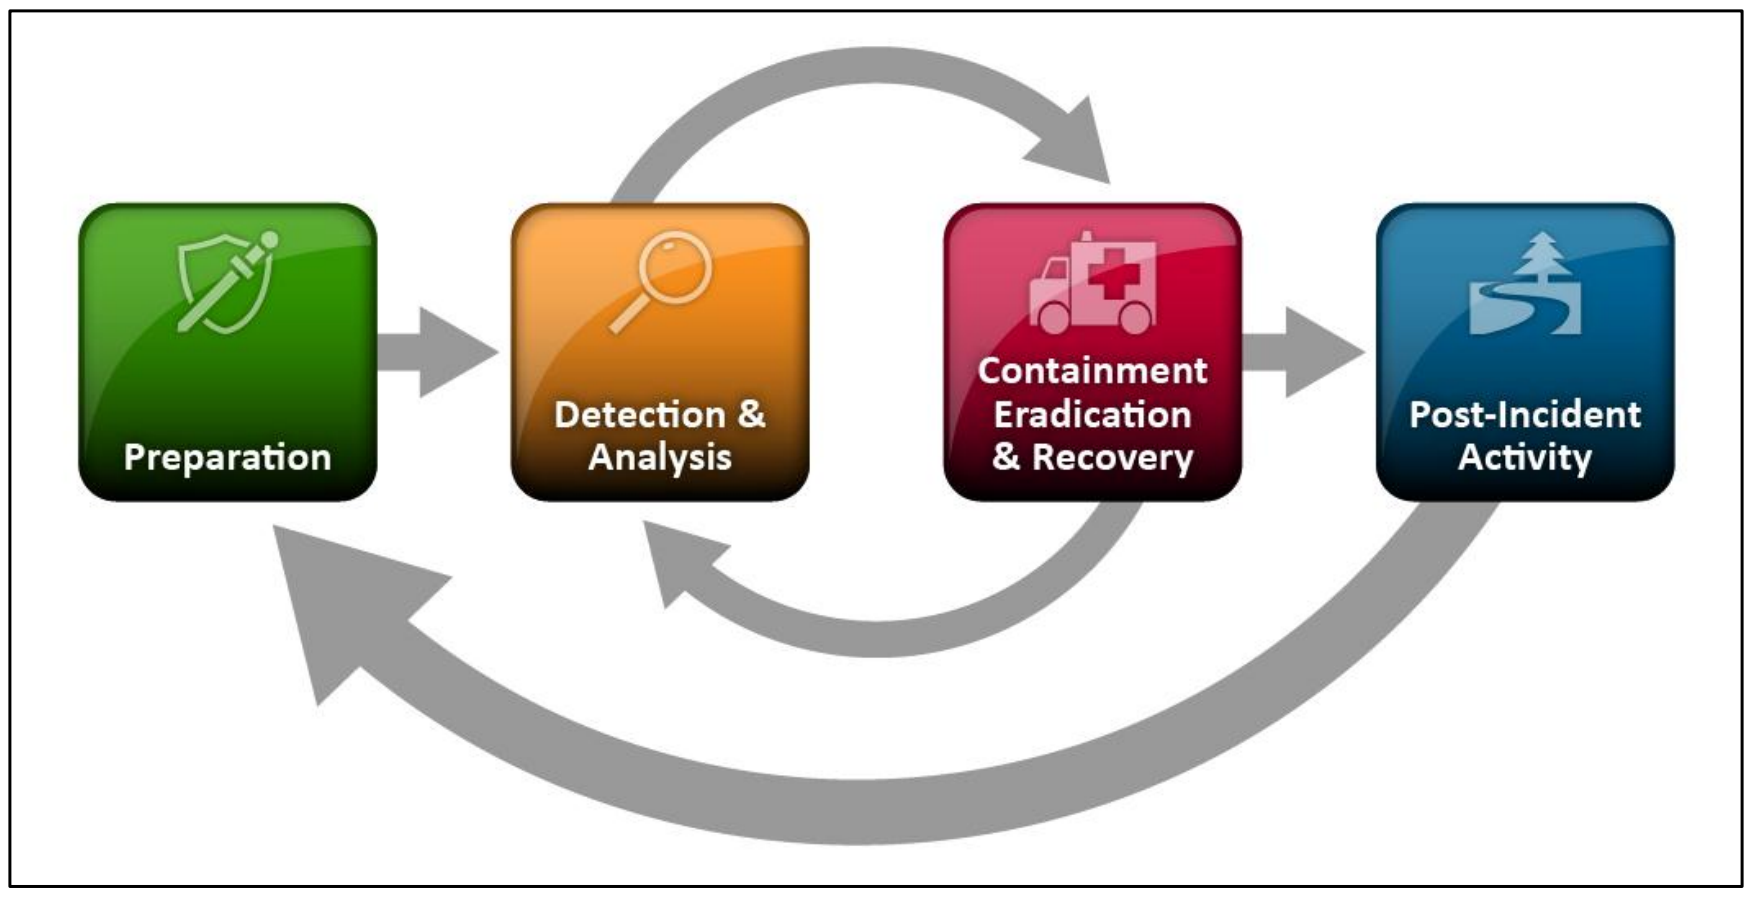
\includegraphics[scale=0.27]{NISTIncidentResponseCycle.png}
\caption[The Incident Response Life Cycle]{The Incident Response Life Cycle \cite{nist800-61}}
\label{fig:NISTIncidentResponse}
\end{center}
\end{figure}

\paragraph{Preparation} 
This phase includes establishing an incident response capability as well as preventing incidents. The latter is not typically a part of the incident response team's tasks, but it is fundamental to the success of the organization's incident response. If a large number of incidents occur, it may overwhelm the incident response team. To prepare for incidents the incident handlers should have tools and resources like contact information, incident reporting mechanisms, issue tracking system, digital forensic workstations\footnote{A digital forensic workstation is specially designed for acquiring and analysing data. It usually contains a set of removable hard drives that can be used for evidence storage.} and digital forensic software. It is common to create a portable \emph{jump kit} containing materials that may be needed during incident response.

\paragraph{Detection and Analysis}
Organizations should prepare to handle any type of incident and to handle common incident types. A classification of incidents can be used as a basis for incident handling. The guidelines provides a list of example categories for incidents that contains web, email, improper usage and loss or theft of equipment. This guidelines focuses on handling of any type of incident and not specific categories. A challenge related to incident handling is to detect the incident and determine the potential impact the incident may have. The actual detection may be the hardest part of incident handling. The guidelines defines two types of signs of incidents; precursors and indicators, with indicators being the most common. These are defined in the following way: "A \emph{precursor} is a sign that an incident may occur in the future. An \emph{indicator} is a sign that an incident may have occurred or may be occurring now." Common sources for precursors and indicators are \acp{IDPS}, antivirus and antispam software, third-party monitoring services, logs, information on new vulnerabilities and exploits and people. 

A challenging part of this phase is the analysis, i.e. to determine which indicators and precursors are legitimate, if they are really related to an incident and what has actually happened. When the team believes an incident to have occurred they should try to determine the scope. All steps taken should be documented and timestamped. It is important to note that any such documentation can be used in court. The incident response team should maintain a database containing information about incidents, such as status, indicators, related incidents and actions taken by the incident handlers. It is important to prioritize incidents and handle them accordingly. Factors that can be used as a basis for prioritization include the functional impact of the incident, the information impact of the incident and recovery from the incident. When the prioritization is performed the incident response team should notify the appropriate people. It is important to have procedures regarding who these people should be.

\paragraph{Containment, Eradication and Recovery}
Containment is obviously an important part of incident handling. The existence of strategies and procedures for containment is helpful. These strategies and procedures are different for different types of incidents. Gathering and handling of evidence is part of this phase. For some incidents eradication is necessary and for some it is done during recovery. Eradication can include deleting malware and disabling breached user accounts. Recovery consists of restoring systems to normal operation and in some cases eliminate vulnerabilities that could have causes similar incidents. The guidelines does not offer specific recommendations for eradication and recovery as these are often OS specific. 

\paragraph{Post-Incident Activity}
Learning and improving is one of the most important parts of incident response. It is recommended to hold a ``lessons learned" meeting after each major incident and periodically after lesser incidents. One meeting could cover several incidents. ``Lessons learned" meetings should generally focus on revealing what was done well and what could be improved. The desired result is that the organization will be better equipped for the next incident that occurs. Often incident response policies and procedures are updated. The areas these meetings should focus on include how well the staff performed and what they could have done differently, if documented procedures were followed and if they were adequate and how information sharing with other organizations could have been improved. To prevent future similar incidents potential corrective actions and potential additional tools and resources should be reviewed. Both people involved in the incident(s) in question and people needed for future cooperation should be included in these meetings. A follow-up report that provides a reference that can be used when handling future similar incidents should be created. Other post-incident activities include the use of collected data for risk assessment, measurement processes to determine the success of the incident response team and audits of incident response programs. 





\section{Related Work}